\chapter{物理节点单故障可生存性虚拟网络嵌入算法}
\section{问题描述}
在这一部分中,我们首先介绍了虚拟网络嵌入的基本概念,然后提出了我们的可生存虚拟网络嵌入问题。
\subsection{虚拟网络嵌入}
我们将\textbf{虚拟网络}VN表示为无向图$G (V,E)$,其中$V$和$E$分别是虚拟节点和虚拟链路的集合。每个虚拟链路$e_{ij}$具有带宽需求$d_{ij}$。每个虚拟节点$v_i$具有计算容量需求$d_i$。对于虚拟节点$v_i$,需要在虚拟节点上执行的虚拟函数表示为$f(i)$。如图\ref{fig:VirtualNetworkRequest}所示虚拟网络$G (V,E)$ 具有虚拟节点集$V=\{v_1,v_2,v_3,v_4\}$和虚拟边集$E= \{e_{12},e_{13},e_{14},e_{23}\}$。需要在这些虚拟节点上执行的虚拟函数是$f(1)=f_1$, $f(2)=f_2$, $f(3)=f_3$, $f(4)=f_4$。

\begin{figure*}
\centering
% Requires \usepackage{graphicx}
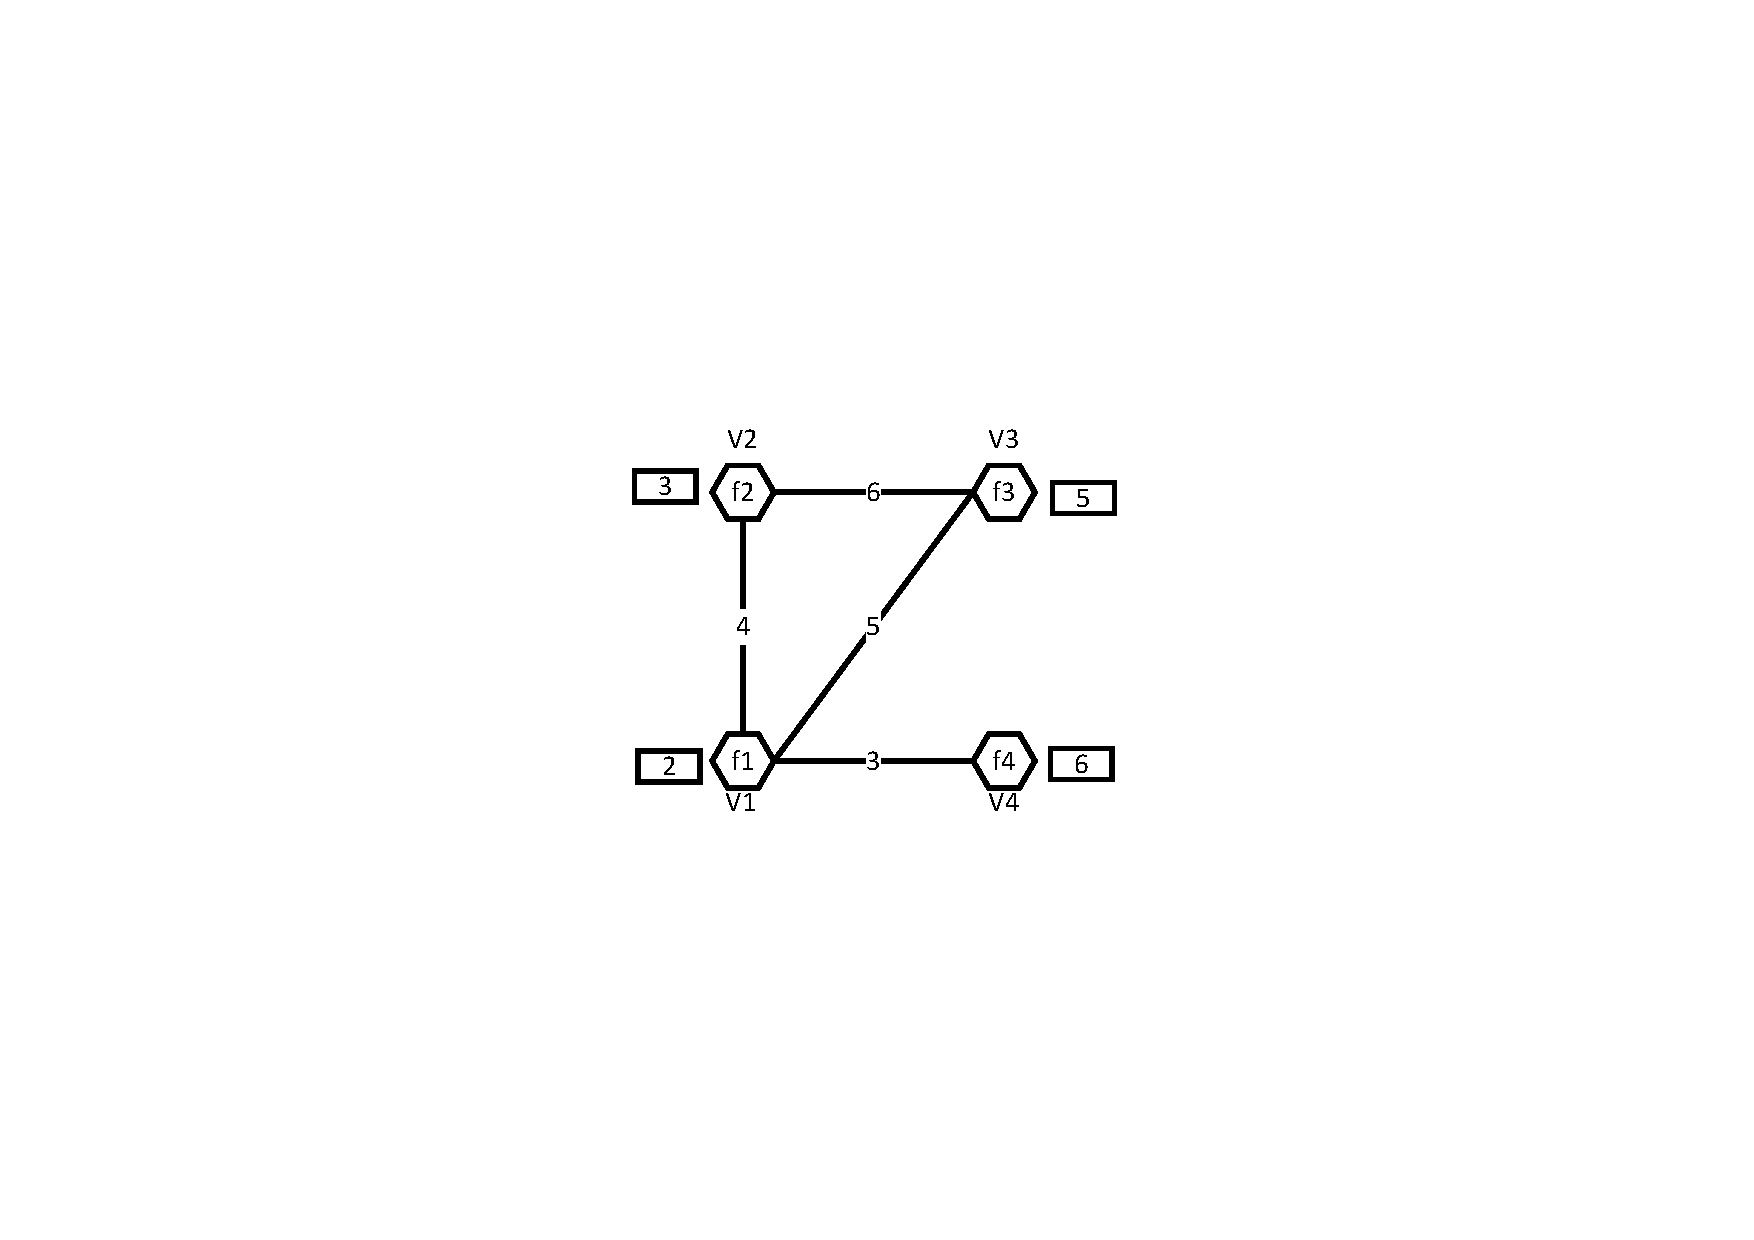
\includegraphics[width=4in]{figures/VirtualNetworkRequest}\\
\caption{虚拟网络请求$G(V,E)$, $V=\{v_1,v_2,v_3,v_4\}$, $E=\{e_{12},e_{23},e_{13},e_{14}\}$,  $f(i)=\{f_1,f_2,f_3,f_4\}$, $d_i=\{2,3,5,6\}$, $d_{ij}=\{4,5,3,6\}. $
}\label{fig:VirtualNetworkRequest}
\end{figure*}

我们将底层\textbf{物理网络}建模为一个无向图$G (S,L)$,其中$S$和$L$分别是物理节点和物理链路的集合。对于物理节点$s_i$,我们使用$F(i)$和$c_i$分别表示可以在该节点上执行的一组可行的虚拟功能和可用的计算能力。每个物理链路$l_{ij}$ 都有可用带宽$b_{ij}$。如图\ref{fig:PhysicalNetwork}所示的物理网络$G (S,L)$,物理节点集合$S=\{s_1,s_2,s_3,s_4,s_5,s_6,s_7,s_8\}$,链路集合$L=\{l_{12},l_{13},l_{14},l_{15},l_{23},l_{25},l_{35},l_{36},l_{37},l_{47},l_{58}\}$,
每一个物理节点的可行的虚拟功能$F(1)=\{f_1\}$, $F(2)=\{f_2,f_3\}$, $F(3)=\{f_3\}$, $F(4)=\{f_4\}$, $F(5)=\{f_1,f_2\}$, $F(6)=\{f_1,f_4\}$, $F(7)=\{f_2,f_3\}$,$F(8)=\{f_2\}$。

\begin{figure*}
\centering
% Requires \usepackage{graphicx}
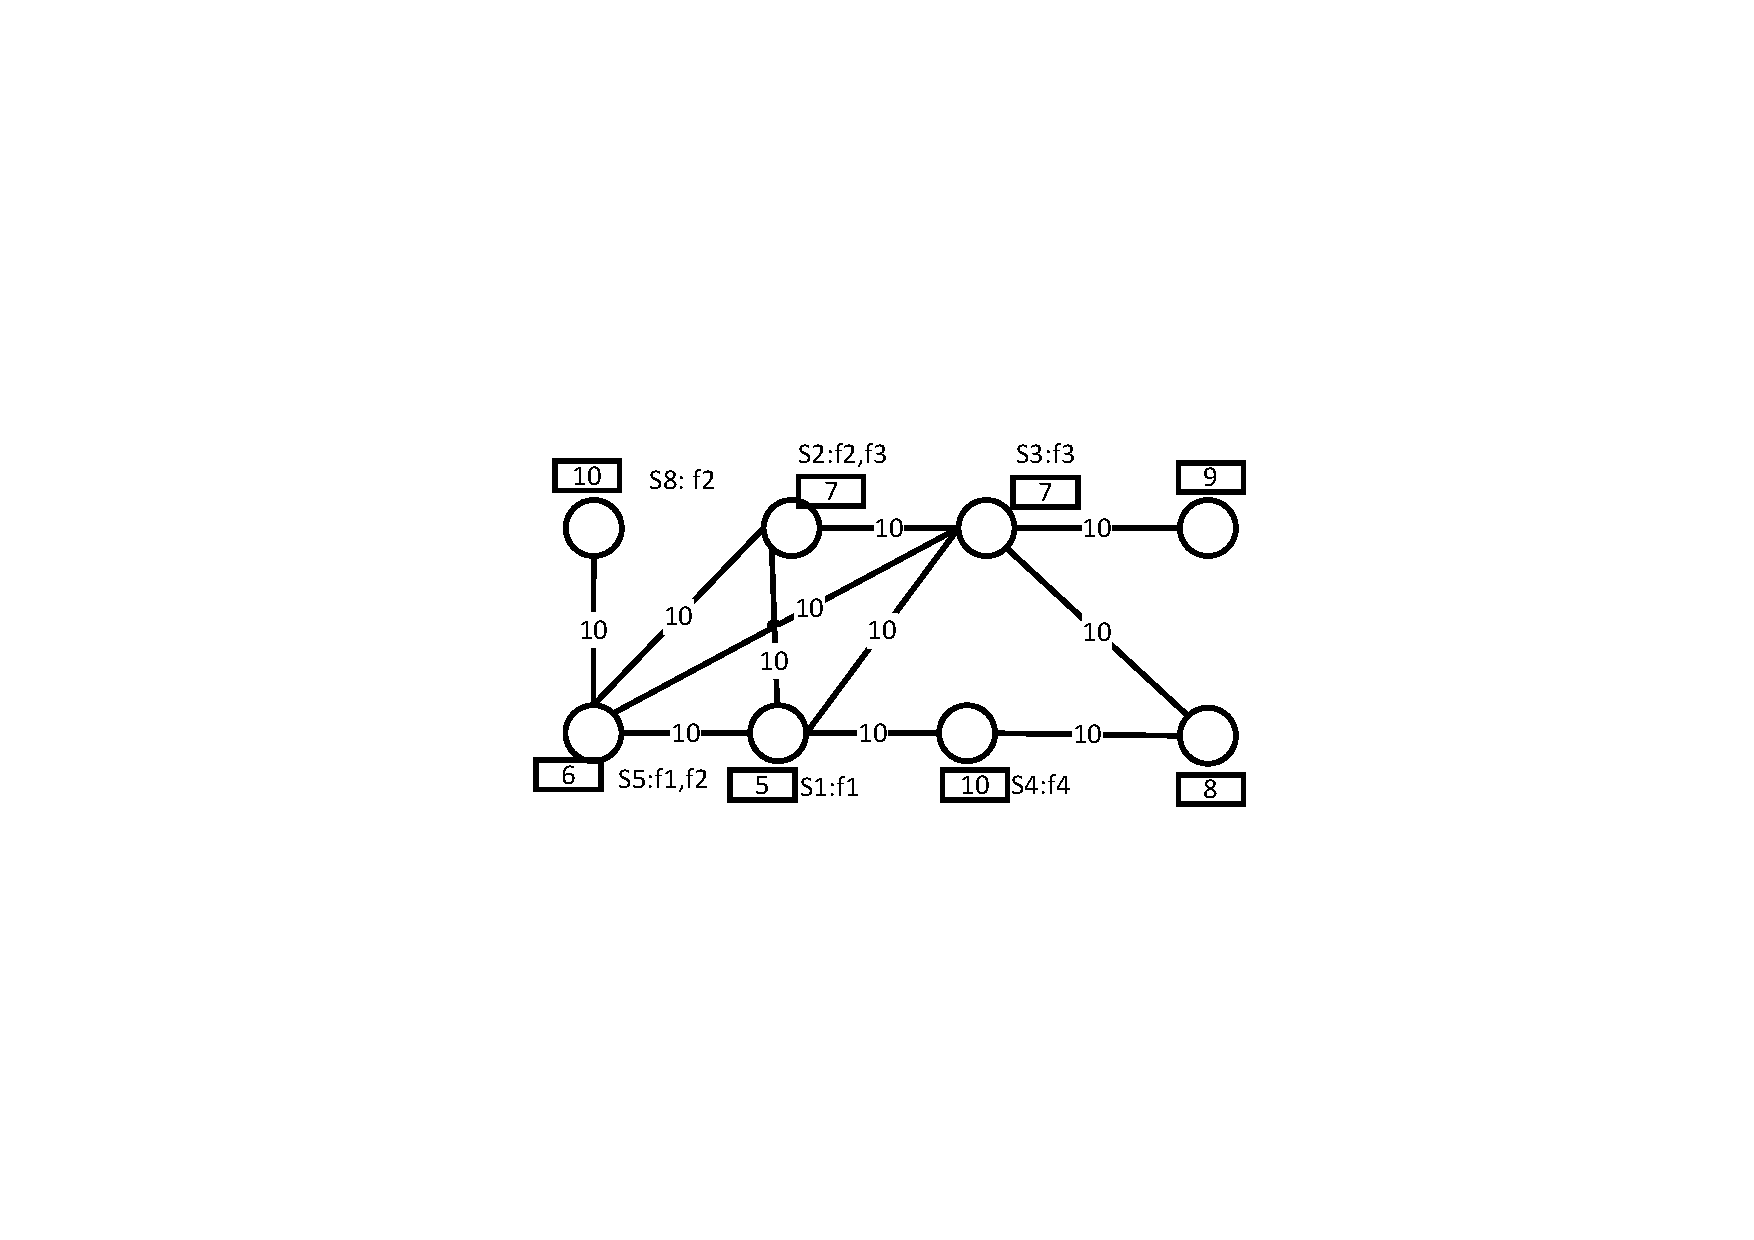
\includegraphics[width=4in]{figures/PhysicalNetwork}\\
\caption{底层物理网络$G(S,L), S=\{s_1,s_2,s_3,s_4,s_5,s_6,s_7,s_8\}, L=\{l_{12},l_{13},l_{14},l_{15},l_{23},l_{25},l_{35},l_{36},l_{37},l_{47},l_{58}\}, F(i)=\{\{f_1\},\{f_2,f_3\},\{f_3\},\{f_4\},\{f_1,f_2\},\{f_1,f_4\},\{f_2,f_3\},\{f_2\}\}, c_i=\{5,7,7,10,6,9,8,10\}, b_{ij}=\{10,10,10,10,10,10,10,10,10,10,10\}$}\label{fig:PhysicalNetwork}
\end{figure*}

在给定VN请求$G (V,E)$的情况下,虚拟网络嵌入问题的目的是将该请求映射到物理网络$G (S,L)$ 上,同时提供所需的足够资源。一个可行的嵌入应该满足节点容量约束、链路带宽约束和功能类型约束这三个约束条件。

对于一个虚拟节点$v_i$,物理节点$s_j$只在节点容量约束和功能类型两种情况满足约束条件(即${f_i} \in {F_j}$)下被映射这个虚拟节点。即节点的容量请求应满足$d_i\leq c_j$的物理节点,虚拟节点上需要执行的虚拟功能属于物理节点$s_j$上可以执行的虚拟功能${f_i} \in {F_j}$。如果物理节点$s_j$满足这两个约束,则节点映射是可行的,并且我们表示这样的映射为$\phi ({v_i}) = {s_j}$。

对于在两个已经映射到两个物理节点$s_{i'}$和$s_{j'}$(即$\phi({v_i}) = {s_{i'}}$和$\phi({v_j}) = {s_{j'}}$) 的虚拟节点之间的虚拟链路$e_{ij}$,在链路带宽约束下$d_{ij}\leq b_{i'j'}$(其中$b_{i'j'}$是连接物理节点$s_{i'}$和$s_{j'}$的可用带宽),这条虚拟链路$e_{ij}$可以映射到物理路径$p_{\phi({v_i}) \phi({v_j})}$,则表示可行的链路映射为$\rho(e_{ij}) = p_{\phi({v_i}) \phi({v_j})}$。

显然,为了找到一个可行的虚拟网络嵌入,我们需要找到两个映射函数$\phi$ 和$\rho$来将所有虚拟节点映射到物理节点,以及将所有链路链接映射到物理路径。

如图\cite{fig:VirtualNetworkEmbedding}所示一个可行的虚拟网络嵌入,将图\cite{fig:VirtualNetworkRequest}中的虚拟网络嵌入到图\cite{fig:PhysicalNetwork}中的物理网络中,其中虚拟节点$v_1$嵌入到物理节点$s_1$,虚拟节点$v_2$嵌入到物理节点$s_2$,虚拟节点$v_3$嵌入到物理节点$s_3$,虚拟节点$v_4$嵌入到物理节点$s_4$。在图\ cite{fig:PhysicalNetwork}中,我们还展示了在这样的映射之后物理网络中已经占用的和可用的资源。例如,对于物理节点$s_1$,其占用的计算容量为2,可用容量为5。

给定VN请求$G(V,E)$和物理网络$G(S,L)$,对于可行映射,我们将映射的物理图表示为$G\left( {\hat S,P} \right)$,其中$\hat S$是容纳虚拟节点的物理节点集,其中$\hat S = \{ {s_{i'}}:\phi({v_i}) = {s_{i'}},for\ \ {\rm{ }}all\ {v_i} \in V,{s_{i'}} \in S\}$ 和$P$是路径集,其中每个路径都持有一个虚拟链路$P = \{ p_{\phi({v_i}) \phi({v_j})}:\rho(e_{ij}) = p_{\phi({v_i}) \phi({v_j})}{\rm{ }}, for\ all,{e_{ij}} \in E\}$。由于每个虚拟链路对应一个物理网络路径,该路径由多个物理链路组成,因此我们还将$G\left( {\hat S,\hat L} \right)$表示为占领的物理网络$\hat L = \{ {l_{pg}}:{l_{pg}} \in {p_{s_{i'}s_{j'}}}, \rho(e_{ij}) = p_{\phi({v_i}) \phi({v_j})},for\ all\ {e_{ij}} \in E,{l_{pg}} \in L\}$。

已经有了许多研究虚拟网络嵌入问题\cite{fischer2013virtual};,因为本文的重点不是虚拟网络嵌入算法,我们采用了\cite{lischka2009virtual}中的算法作为基本的虚拟网络嵌入算法。


\begin{figure*}
\centering
% Requires \usepackage{graphicx}
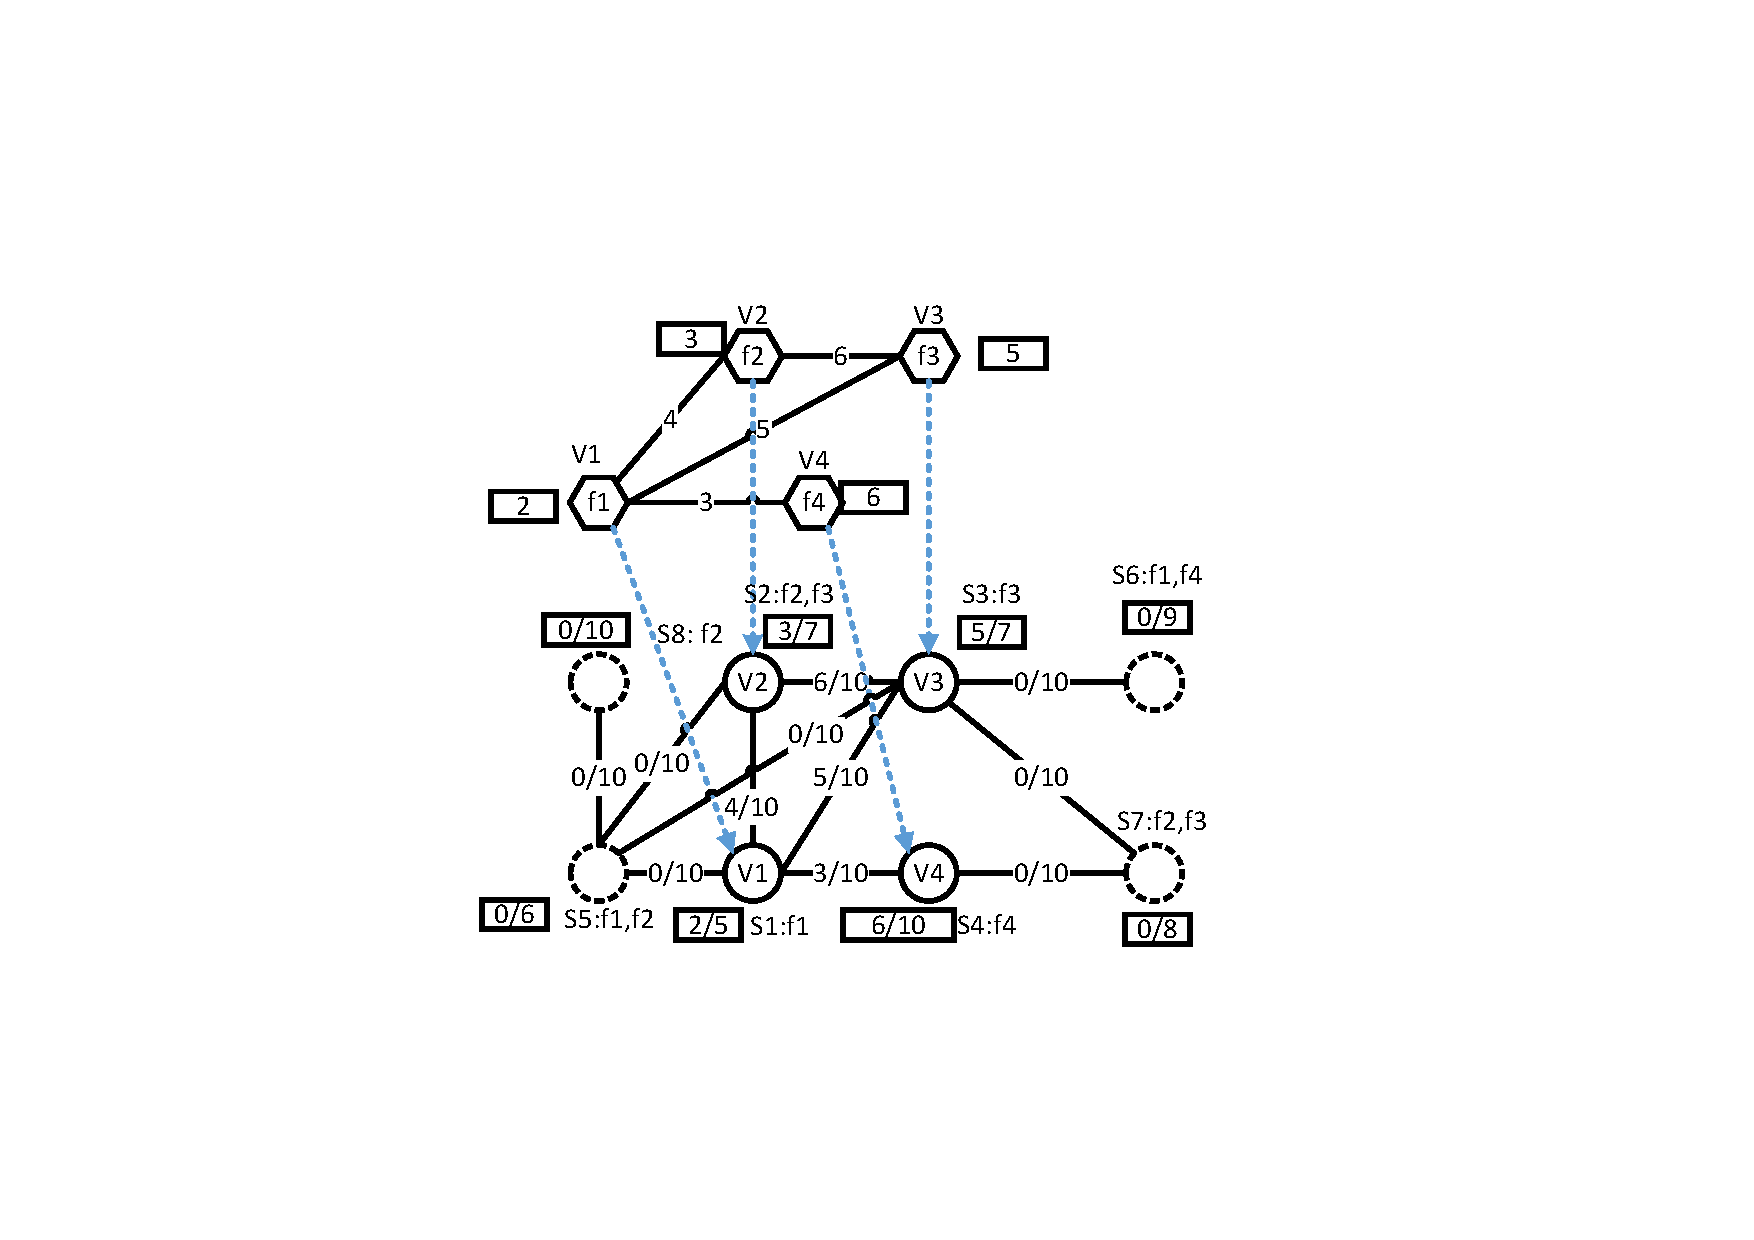
\includegraphics[width=4in]{figures/VirtualNetworkEmbedding}\\
\caption{节点映射$v_1\rightarrow s_1, v_2\rightarrow s_2, v_3\rightarrow s_3, v_4\rightarrow s_4$,链路映射$e_{12}\rightarrow l_{12},e_{23}\rightarrow l_{23},e_{13}\rightarrow l_{13},e_{14}\rightarrow l_{14}$.}\label{fig:VirtualNetworkEmbedding}
\end{figure*}
\subsection{可生存性虚拟网络嵌入}
由于恶意攻击、自然灾害、无意中断电缆、计划维护、设备故障、物理节点承载的虚拟节点可能会遭受不可避免的故障。当单个或多个物理网络组件发生故障时,VN中可能会发生故障,从而造成财务损失。一般来说,多个物理节点的同时失效是相互独立的,单个节点的失效通常发生在大多数时间\cite{yeow2010designing}。本文研究了单节点失效的可生存虚拟网络嵌入问题。在本章中,我们将讨论如何将我们的算法扩展到多节点故障的场景中。

对于VN请求$G (V,E)$和物理网络$G (S,L)$,给出了其占用物理网络的可行映射,在任何一个物理节点发生故障时,增加最小备份物理资源以提供可生存性的网络服务。

节点故障不仅影响运行在失效的物理节点上的可视化服务,而且会终止通过该节点的所有通信。物理节点 $ {s_i} \in S $的失效导致相邻物理链路的失效${L_i} = \left\{ {{l_{ik}}:k \in N(i)} \right\}$,其中${N(i)}$是节点$ {s_i} $的邻居节点。

由于我们无法预测哪个节点将失效,即使我们知道多个节点不会同时失效,为了处理单节点故障,一个直接的方式是为VN请求中的每个虚拟节点提供专用备份资源,也称为1+1保护方案。如图\cite{fig:One2OneProtection}所示利用一个例子来说明这种直截了当的方法。在该示例中,将具有4个虚拟节点的虚拟网络映射到物理网络,其中4个物理节点参与了这样的嵌入。为了提供1 +1保护方案,在图中添加了4个备份节点、8 个备份链路。

1+1保护方案虽然实现简单,但需要大量的备份资源.我算法的目的是以最小的备份资源成本提供可生存的网络服务。

\begin{figure}
\centering
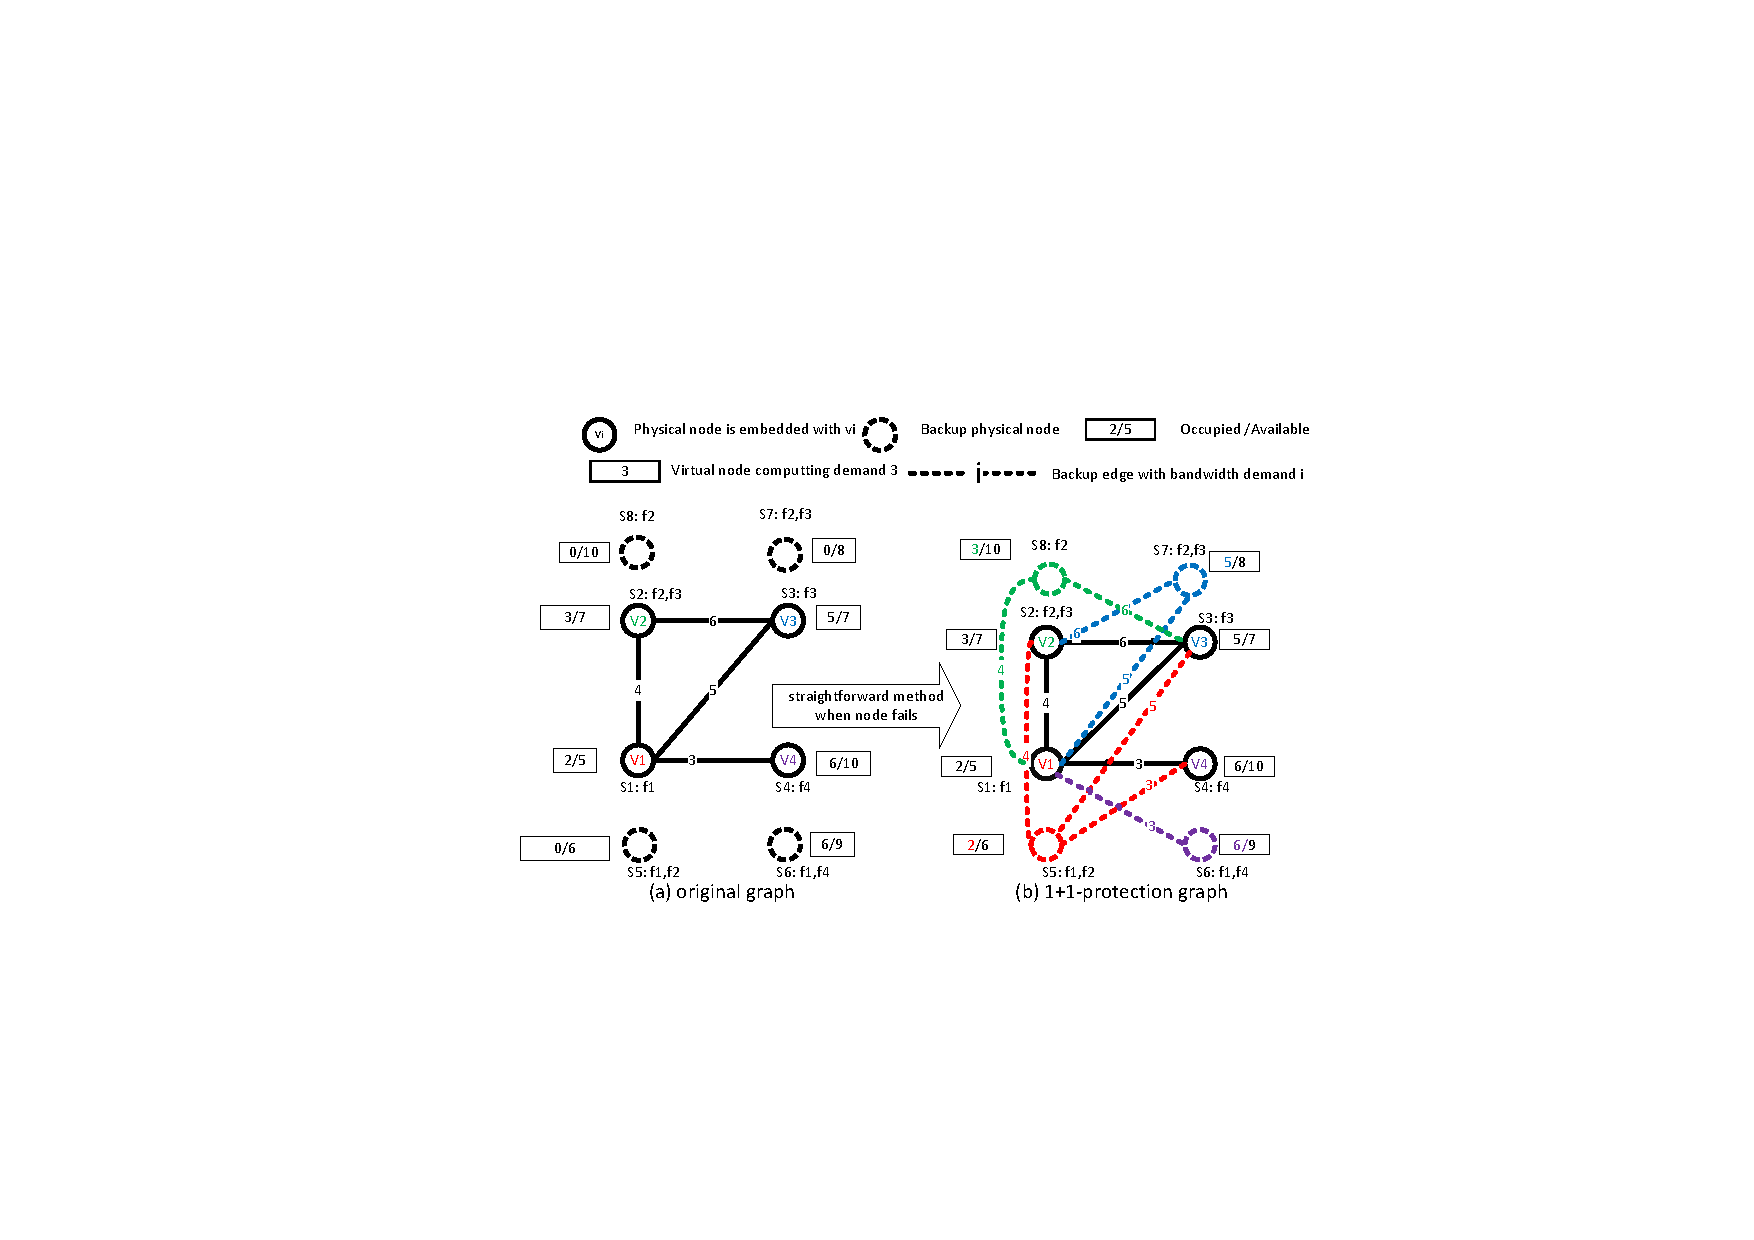
\includegraphics[width=3.5in]{figures/One2OneProtection}\\
\caption{1+1-保护机制}\label{fig:One2OneProtection}
\end{figure}
\section{基于问题公式的图分解}
可生存虚拟网络嵌入需要添加备份资源,以保证当任何一个物理节点失败时,剩余的物理资源加上备份资源仍然可以支持可行的映射。为了便于在节点失败时找到可行的映射,本节首先对虚拟网络进行分解。物理网络以星型为基础的局部组件。在此基础上,提出了一种新的二部图,并将具有最小备份资源的可生存虚拟网络嵌入问题转化为一个基于定义良好的二部图的虚拟星图分配问题。
\subsection{星型图分解}

\subsection{二分图}

\section{动态分配}
\section{算法性能评估}
\section{本章小节}
